\documentclass{article}

\usepackage{fullpage,verbatim,amsmath,graphicx}

\newcommand{\HRule}{\rule{\linewidth}{0.5mm}}
\begin{document}

\begin{titlepage}
 
\begin{center}
 
\textsc{\LARGE Homework 3}\\[1.5cm] 

\textsc{\Large Computational Math}\\[0.5cm]
 
 
\HRule \\[2cm]
 
% Author and supervisor
\begin{minipage}{0.4\textwidth}
\begin{flushleft} \large
\emph{Author:}\\
Mikola Lysenko
\end{flushleft}
\end{minipage}
 
\vfill
 
% Bottom of the page
{\large \today}
 
\end{center}
 
\end{titlepage}


\paragraph{1} Asymptotically, the cost of multiplying an $n\times n$ matrix by a vector is $O(n^2)$, while the time complexity of chebfft.m is dominated by the cost of the Fourier transform, which is $O(n \log(n))$.  However, due to cache performance issues and other numerical overhead, the constant for chebfft.m is much higher, and so one should expect that for small values of $n$, cheb.m ought to be faster.  To compare the performance of the two methods, I wrote the following MATLAB code to estimate their performance:

\begin{verbatim}
N = 1024;
K = 64;
P = 16;
fft_times = zeros(N,1);
bf_times = zeros(N,1);
data = zeros(K,1);
for n=2:N
    [D,x] = cheb(n);
    for k = 1:K
        tic;
        for p = 1:P
            chebfft(x);
        end
        data(k) = toc / P;
    end
    fft_times(n) = median(data);
    for k = 1:K
        tic;
        for p = 1:P
            xx = D * x;
        end
        data(k) = toc / P;
    end
    bf_times(n) = median(data); 
end
plot( 2:N, fft_times(2:N), 2:N, bf_times(2:N) );
\end{verbatim}

The codes were run multiple times in order to smooth out potential problems due to individually bad runs (ie most likely caused by CPU thrashing due to my impatience and working on other homework).  The effects of noise became more pronounced as the time of the computation grew longer.  The median filtering is intended to smooth out these problems and give a better estimate for the actual performance of the method instead of the somewhat raw estimate obtained via brute-force sampling.  Here is a graph of the resulting smoothed plots:

\begin{center}
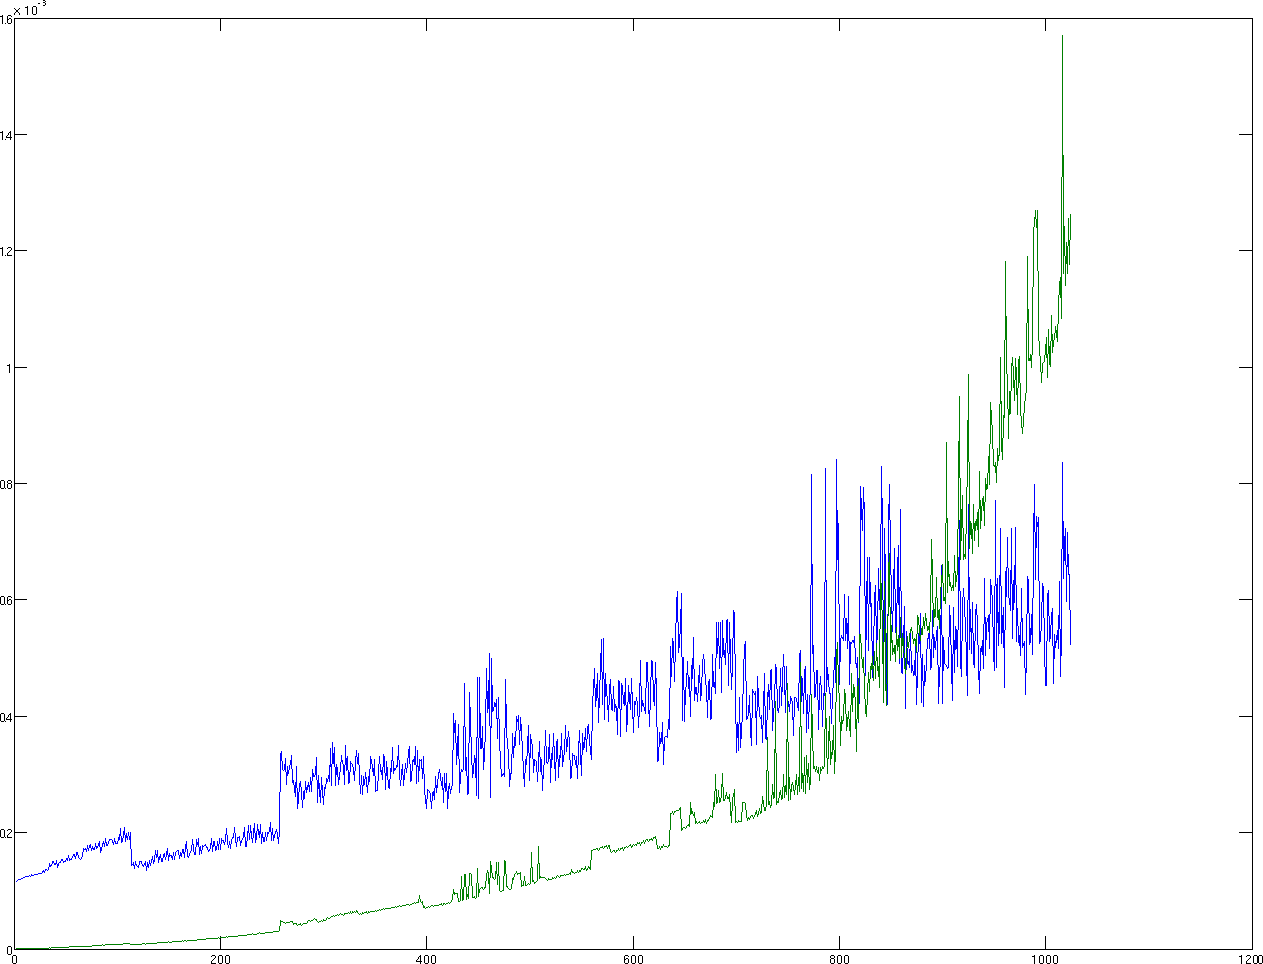
\includegraphics[width=2in]{plot1.png}
\end{center}

By inspection, it appears that for $n > 800$ the FFT method is faster, while for smaller values the brute-force matrix multiplication performs better.  With a more optimized implementation of chebfft, this value could possibly be lowered.

\paragraph{2}  
Here is my modified code for the matrix based method:

\begin{verbatim}
  dt = 6/N^2;
  [D, x] = cheb(N);
  y = x';
  D2 = dt^2 * (D * D);
  D2(1,:) = 0;
  D2(N+1,:) = 0;
  I = eye(N+1);
  L = kron(I, D2) + kron(D2, I);  
  [xx,yy] = meshgrid(x,y);
  vv = exp(-40*((xx-.4).^2 + yy.^2));
  vvold = vv; 
  for n = 0:round(3/dt)
    t = n*dt;
    vvnew = 2*vv - vvold + reshape(L * reshape(vv, (N+1)^2, 1), N+1,N+1);
    vvold = vv; 
    vv = vvnew;
  end
\end{verbatim}

And here is a plot of the results:

\begin{center}
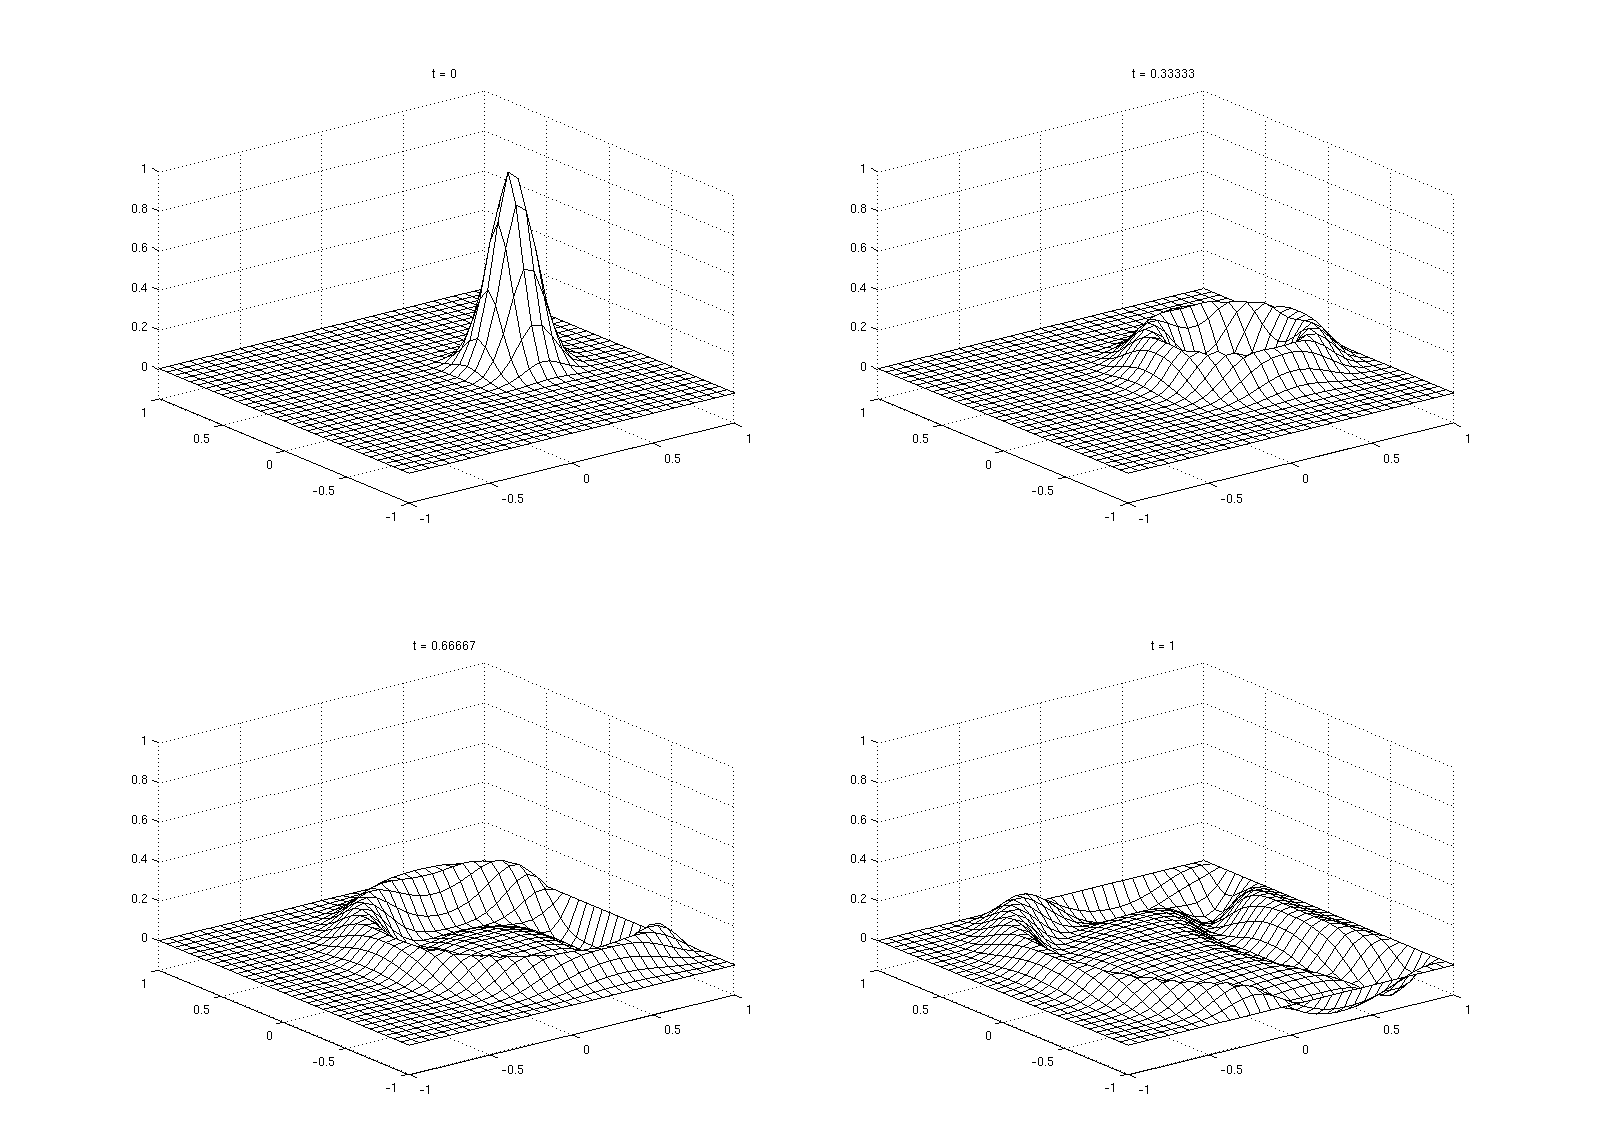
\includegraphics[width=4in]{plot3.png}
\end{center}

On my machine I found that the matrix version was faster up to about $N \approx 30$.

\paragraph{3}
Let $T_n$ and $U_n$ denote the $n^{th}$ Chebyshev function of the first (resp. second) kind.  Then, differentiating $T_n$ in the Gauss-Lobato coordinate system, $x \mapsto \cos(\theta)$ gives:
\begin{eqnarray*}
\frac{d^2}{dx^2} T_n ( \cos(\theta) ) & = & \frac{d^2}{dx^2} \cos(n\theta) \\
 & = & \frac{1}{\sin(\theta)^3} \left( -n^2 \sin(\theta) \cos(n \theta) + n \cos(\theta) \sin(n \theta) \right) \\
 & = & \frac{1}{\sin(\theta)^3} \left( n^2 \sin(\theta) T_n - n \cos(\theta) U_n \right)
\end{eqnarray*}
Unfortunately due to the division by $\sin(\theta)^3$, this formula is degenerate at the end points.  To resolve this issue, we explicitly calculate that:
\[ \frac{d^2}{dx^2} T_n( \pm 1 ) = (\pm 1)^n \frac{n^4 - n^2}{3} \]
Translating this expression into MATLAB gives the following code for chebfft2.m:

\begin{verbatim}
function w = chebfft2(v)
  N = length(v)-1; 
  nn = [0:(N-1) 0 1-N:-1]';
  c = cos((1:N-1)'*pi/N);
  s = sqrt(1. - c.^2);
  V = [v; flipud(v(2:N))];
  B = real(fft(V));
  PT    = real(ifft(1i * nn .* B));
  PTT   = -real(ifft(nn .* nn .* B));
  w = zeros(N+1,1);
  w(2:N) = (s .* PTT(2:N) - c .* PT(2:N)) ./ (s.^3);
  w(1) = sum((nn.^4 - nn.^2) .* B ./ (6. * N));
  w(N+1) = sum((-1).^nn .* (nn.^4 - nn.^2) .* B ./ (6. * N));
\end{verbatim}

To compare the accuracy relative to the explicit matrix calculation, I plotted both the matrix form (green) and the FFT version (red) alongside the input function, $v$ (blue) for the following functions:

\begin{center}
\begin{tabular}{ccc}
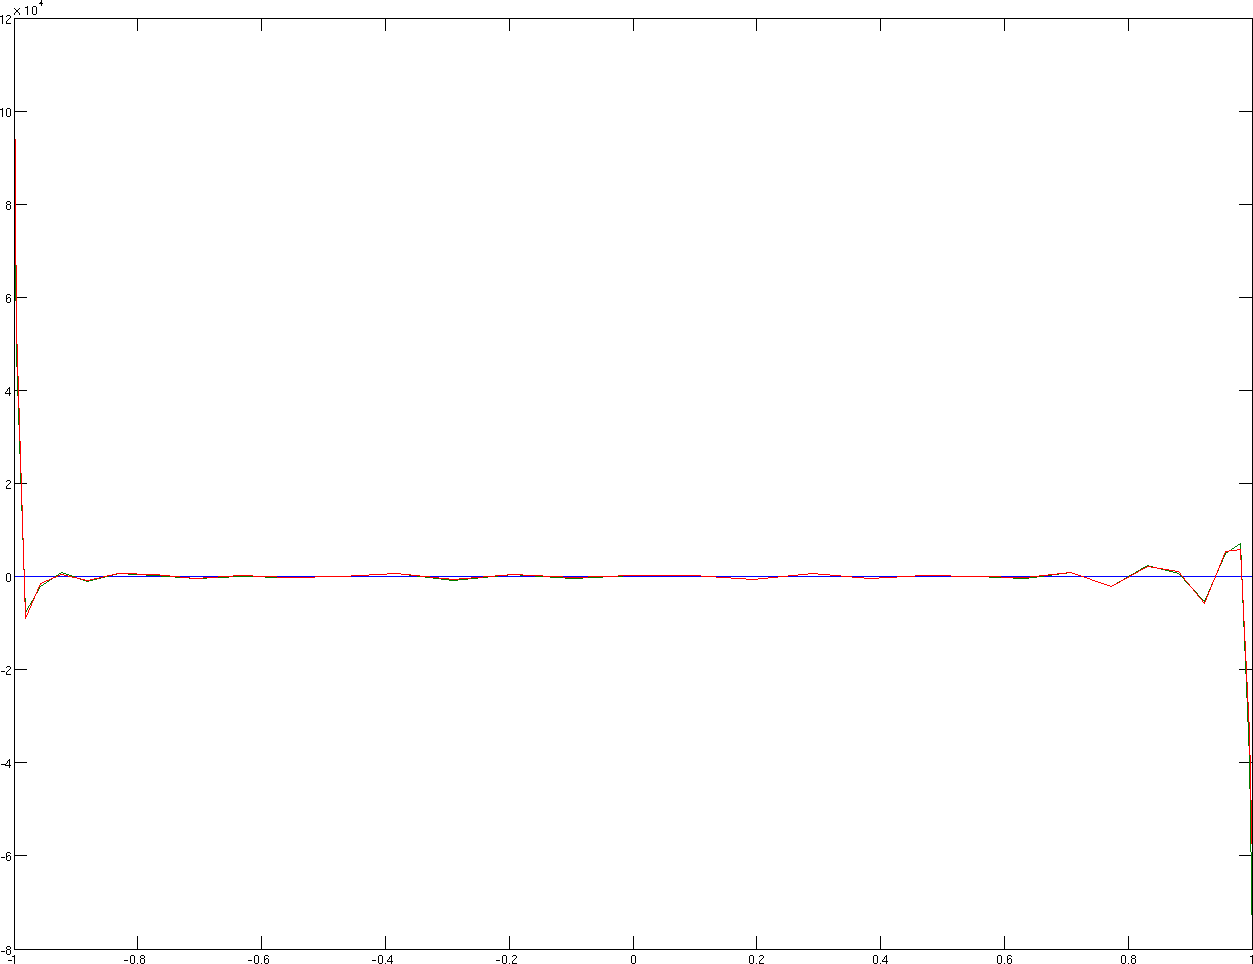
\includegraphics[width=2in]{plot2_1.png} &
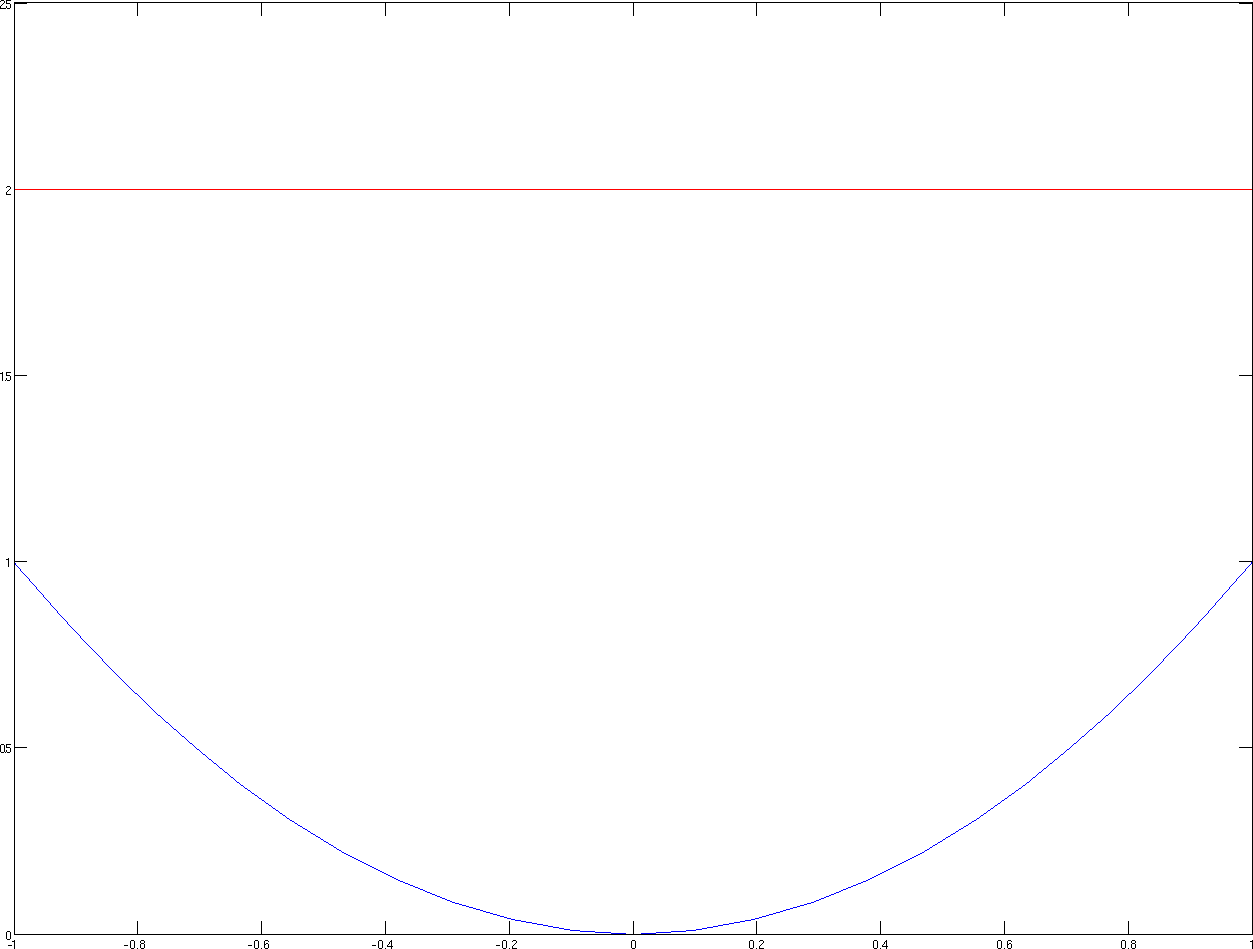
\includegraphics[width=2in]{plot2_2.png} &
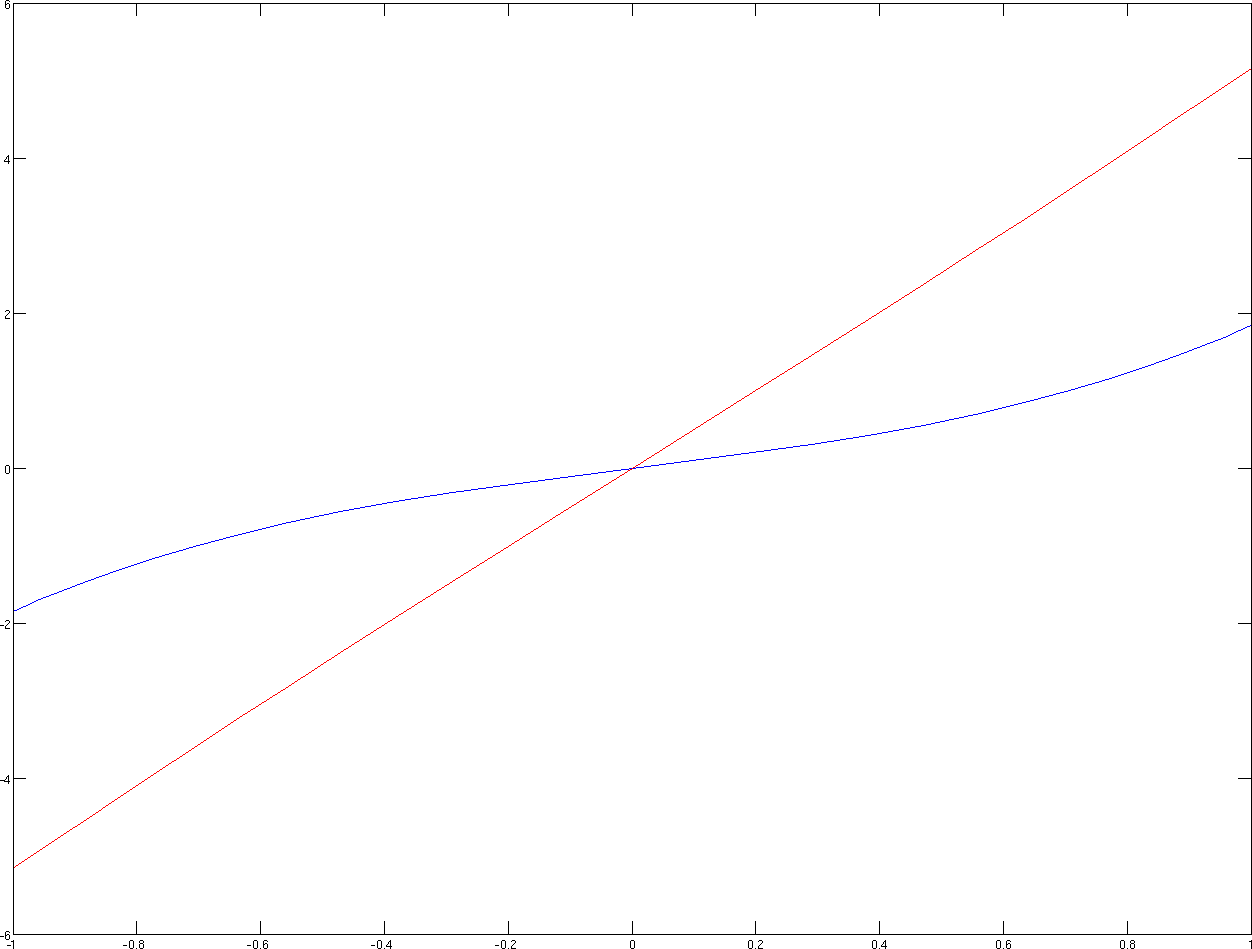
\includegraphics[width=2in]{plot2_3.png} \\
$v = randn$ & $v = x^2$ & $v = x^3 + \sin(x)$ \\
\end{tabular}
\end{center}

\paragraph{4}
Modifying the code was straigthforward.  I just replaced the multiplier, ik3, with
\begin{verbatim}
ik2 = -eps * k.^2;
\end{verbatim}
Here are some plots for various values of $n$:

\begin{center}
\begin{tabular}{ccc}
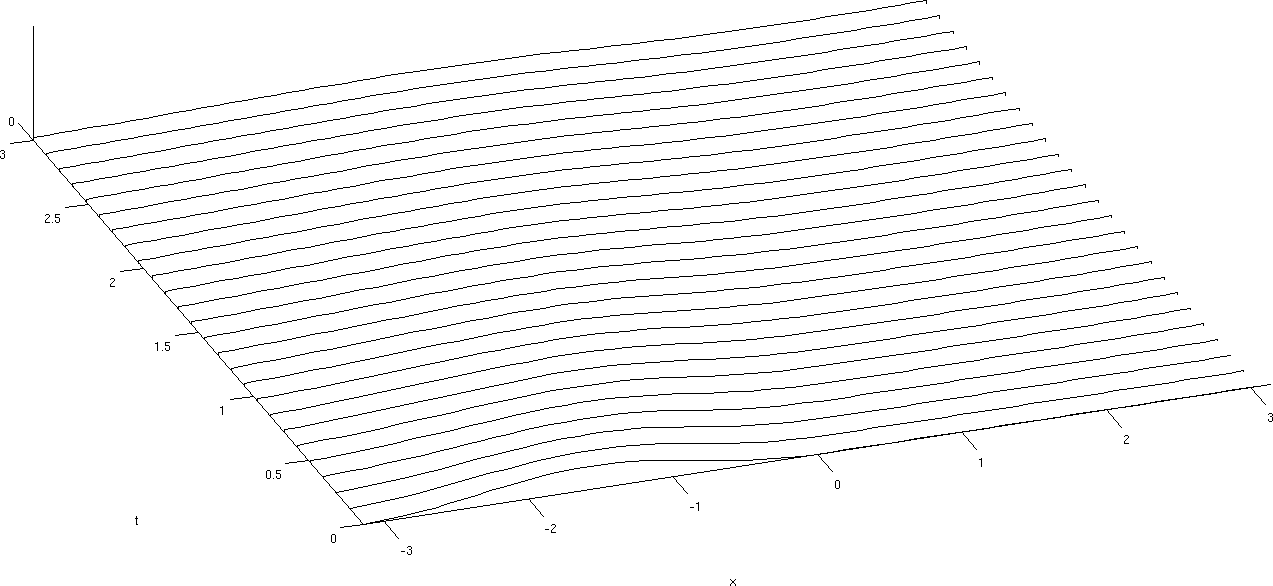
\includegraphics[width=2in]{plot4_1.png} &
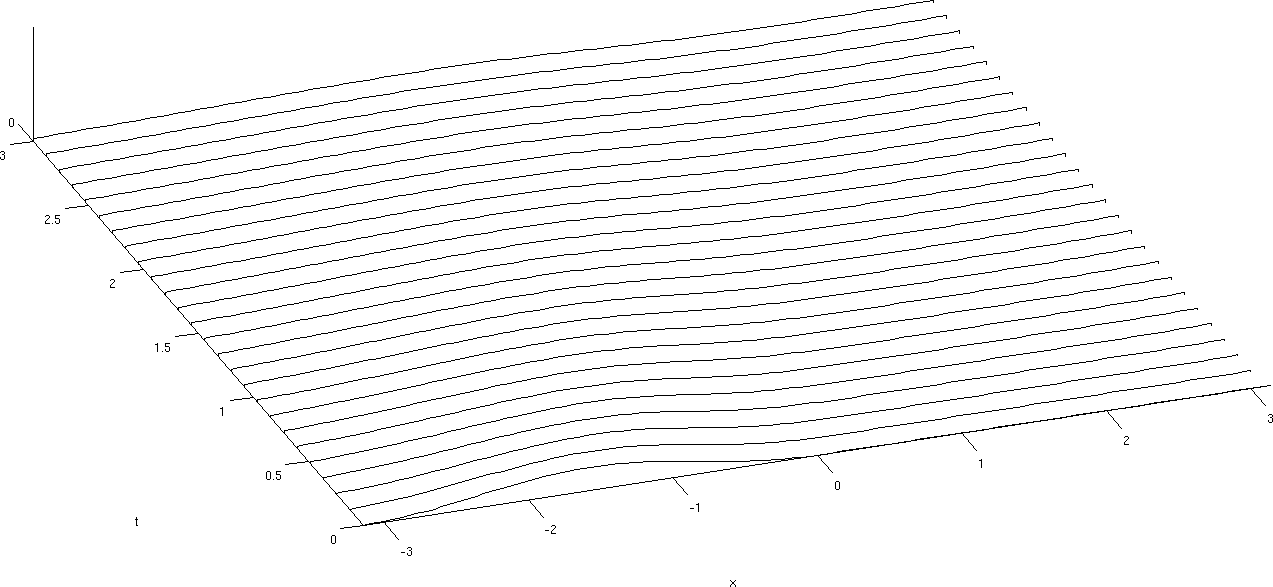
\includegraphics[width=2in]{plot4_2.png} &
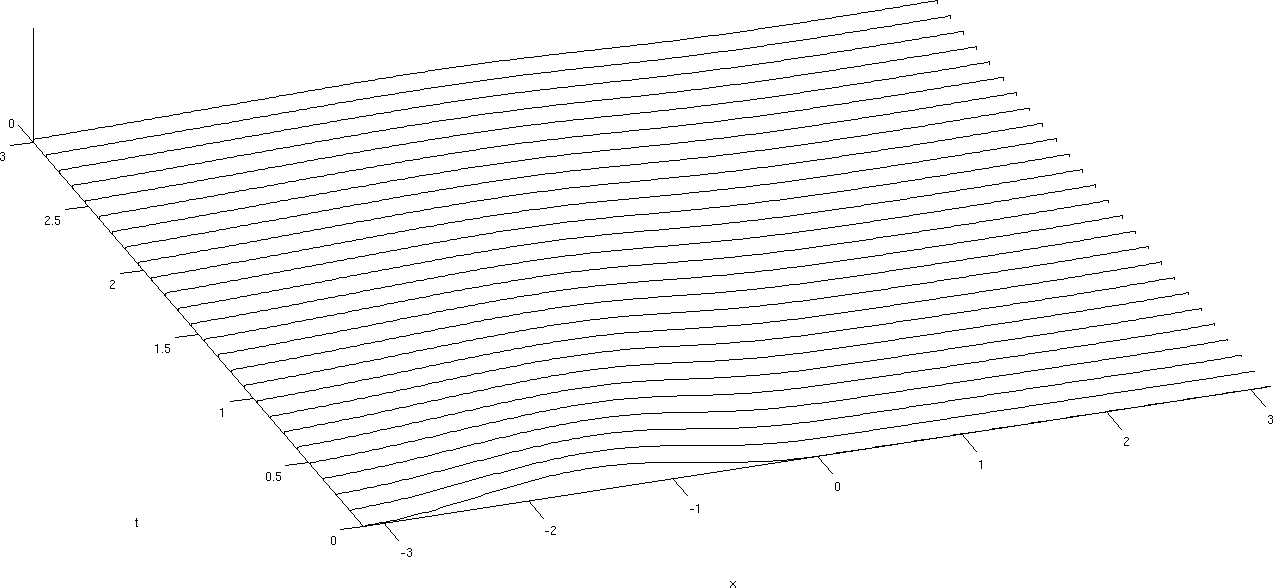
\includegraphics[width=2in]{plot4_3.png} \\
$N = 64$ & $N = 128$ & $N = 256$ \\
\end{tabular}
\end{center}

By experimentation I found that oscillations occured within this interval at $\epsilon \approx 0.05$

\paragraph{5}

Here is my modified version of p20.m :

\begin{verbatim}
  x = (2*pi/N)*(-N/2:N/2-1)';
  A = 25; 
  B = 16; 
  clf, drawnow, set(gcf,'renderer','zbuffer')
  %Initial conditions
  u = exp(-(x .* (20. / pi)).^2);
  v = fft(u); 
  k = [0:N/2-1 0 -N/2+1:-1]'; 
  ik2 = -k.^4 + k.^2;
  tmax = 50.; 
  nplt = floor((tmax/25)/dt); 
  nmax = round(tmax/dt);
  udata = u; 
  tdata = 0; 
  for n = 1:nmax
    t = n*dt; 
    g = -i*dt*k;
    E = exp((.5*dt)*ik2); 
    E2 = E.^2;
    a = g.*fft(real( ifft(     v    ) ).^2);
    b = g.*fft(real( ifft(E.*(v+a/2)) ).^2);     % 4th-order
    c = g.*fft(real( ifft(E.*v + b/2) ).^2);     % Runge-Kutta
    d = g.*fft(real( ifft(E2.*v+E.*c) ).^2);
    v = E2.*v + (E2.*a + 2*E.*(b+c) + d)/6;
    if mod(n,nplt) == 0 
      u = real(ifft(v));
      udata = [udata u]; tdata = [tdata t];
    end
  end
  waterfall(x,tdata,udata'), colormap(1e-6*[1 1 1]); view(-20,25)
  xlabel x, ylabel t, axis([-pi pi 0 tmax 0 1]), grid off
  set(gca,'ztick',[0 10]), pbaspect([1 1 .13])
\end{verbatim}

And here are some plots for various choices of $N, dt$:

\begin{center}
\begin{tabular}{ccc}
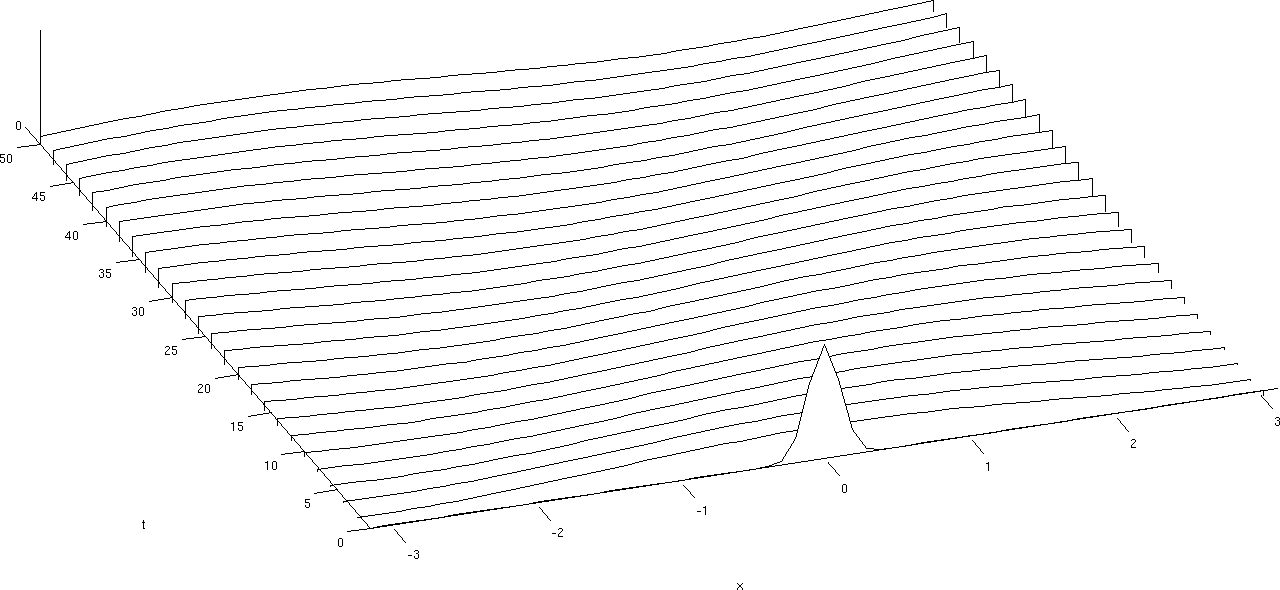
\includegraphics[width=2in]{plot5_1.png}  & 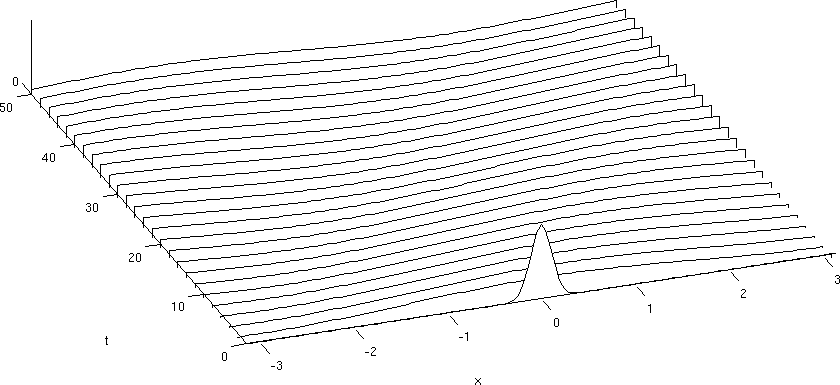
\includegraphics[width=2in]{plot5_2.png} & 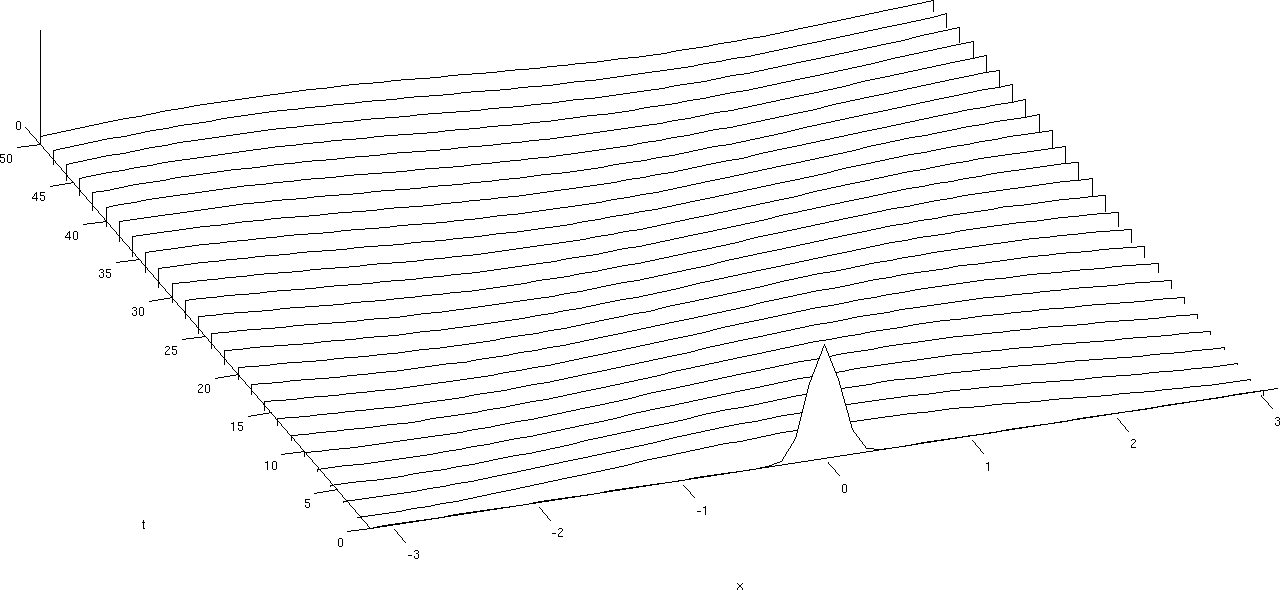
\includegraphics[width=2in]{plot5_3.png} \\
$N=64, dt=10^{-5}$ & $N=128, dt=10^{-5}$ & $N=64, dt=10^{-7}$ \\
\end{tabular}
\end{center}

\end{document}
